\documentclass{beamer}

\usepackage[utf8]{inputenc}
\usepackage{caption}
\captionsetup[figure]{font=scriptsize,labelfont=scriptsize}
% \usepackage{utopia}

\usetheme{Madrid}
\usecolortheme{default}

\title[Deep Reinforcement Learning]{Deep Reinforcement Learning}
\subtitle{Scientific Initiation}
\author[Resck]{Lucas Emanuel Resck Domingues}
\institute[FGV]
{
  Escola de Matemática Aplicada \\
  Fundação Getulio Vargas
}
\date[2020]
{March 2020}

\AtBeginSection[]
{
  \begin{frame}
    \frametitle{Table of Contents}
    \tableofcontents[currentsection]
  \end{frame}
}

\setbeamertemplate{caption}[numbered]

\begin{document}

    \frame{\titlepage}

    \begin{frame}
        \frametitle{Table of Contents}
        \tableofcontents
    \end{frame}

    \section{Introduction}

        \begin{frame}
            \frametitle{Motivation}
        \end{frame}

        \begin{frame}
            \frametitle{Intuition}
        \end{frame}

    % \section{Imitation Learning}

    %     \begin{frame}
    %         \frametitle{Terminology}
    %         At time $t$:
    %         \begin{itemize}
    %             \item $s_t$: the state of the enviroment;
    %             \item $o_t$: the agent observation of the enviroment;
    %             \item $a_t$: the action taken;
    %             \item $\pi_{\theta}(a_t | o_t)$: probability distribution of taken $a_t$ given $o_t$.
    %         \end{itemize}
    %     \end{frame}

    %     \begin{frame}
    %         \frametitle{Imitation Learning goal}
    %         The goal of Imitation Learning is to find a good $\pi_{\theta}(a_t | o_t)$,
    %         in order to take good actions. But it doesn't work.

    %         \begin{figure}
    %             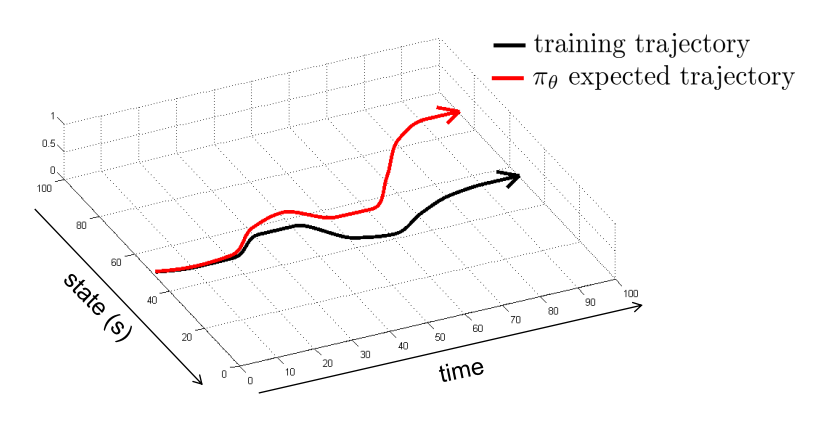
\includegraphics[scale=0.4]{figures/imitation_learning.png}
    %         \end{figure}

    %     \end{frame}

    \section{Reinforcement Learning}

        \begin{frame}
            \frametitle{Markov Decision Process}
            Markov Decision Process is a 4-tuple $(S, A, T, r)$:
            \begin{itemize}
                \item $S$: space of states $s$;
                \item $A$: space of actions $a$;
                \item $T$: transition operator, with probabilities $p(s_{t+1} | s_t, a_t)$
                \item $r$: reward function $r(s, a)$.
            \end{itemize}
        \end{frame}

        \begin{frame}
            \frametitle{The goal of Reinforcement Learning}
            \begin{figure}
                \centering
                \caption{Source: \href{http://rail.eecs.berkeley.edu/deeprlcourse-fa18/static/slides/lec-4.pdf}{Deep RL Berkeley Course}}
                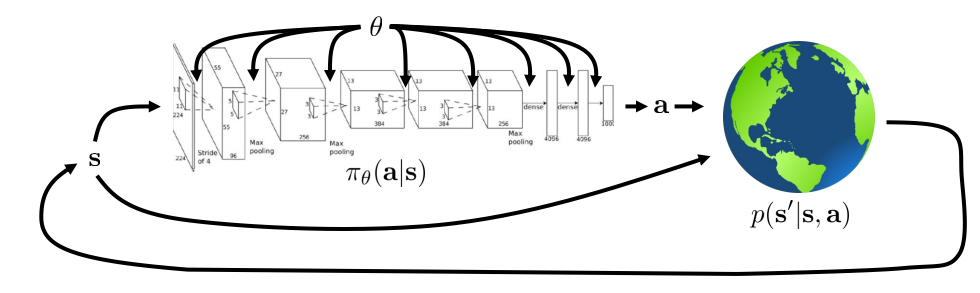
\includegraphics[width=\textwidth]{figures/goal_rl.png}
                \label{fig:1}
            \end{figure}
            $$p_{\theta}(\tau) = p_{\theta}(s_1, a_1, \cdots, s_T, a_T) = p(s_1) \prod_{t=1}^T \pi_{\theta}(a_t|s_t)p(s_t, a_t)$$
            $$\theta^* = \arg\max_\theta E_{\tau \sim p_\theta(\tau)}\left[\sum_t r(s_t, a_t)\right]$$
        \end{frame}

        \begin{frame}
            \frametitle{Too many algorithms}
            \begin{itemize}
                \item Policy iteration;
                \item Value iteration;
                \item Q-learning;
                \item Deep Q-learning.
            \end{itemize}
        \end{frame}

        \begin{frame}
            \frametitle{More definitions}
            \begin{block}{Q Function}
                $$Q^\pi(s_t, a_t) = \sum_{t'=t}^T E_{\pi_\theta}[r(s_{t'}, a_{t'})|s_t, a_t]$$

                The total expected reward for taking an action $a_t$ when the state is $s_t$.
            \end{block}
            \begin{block}{Value Function}
                $$V^\pi(s_t) = E_{a_t \sim \pi_\theta(a_t|s_t)}[Q^\pi(s_t, a_t)]$$

                The total expected reward when the state is $s_t$.
            \end{block}
        \end{frame}

    % Instead of trying to produce a program to simulate the adult mind, why not rather try to produce one which simulates the child's? If this were then subjected to an appropriate course of education one would obtain the adult brain. - Alan Turing
    
\end{document}